% --This template prepared by PRAMOD KUMAR S (pramod.s86@gmail.com) only for reference---
%url:
%www.youtube.com/channel/UCO9kf_V4twFdM4ROdIfy7rw
%www.researchgate.net/profile/Pramod_Kumar3 
%www.linkedin.com/in/pramod-kumar-s-432351141 

% ----------------------Title page--------------------------------------------------
\documentclass[oneside,12pt]{Classes/VTU}
\usepackage{fancyhdr}
\usepackage{Times}


\renewcommand{\submittedtext}{\large{\textbf{\\VISVESVARAYA TECHNOLOGICAL UNIVERSITY }}\\
 Belagavi, Karnataka - 590 018 }

\title{ \normalfont \small{A Project Report on}\\ 
\large{\textbf{PERFORMANCE EVALUATION AND RELIABILITY ANALYSIS OF  PREFABRICATED  CONCRETE STRUCTURES}}}

\degree{Submitted in partial fulfillment of the requirements for the conferment of degree of\\ 
	\textbf{{\large {\\ MASTER OF TECHNOLOGY}}} \\
	 in \\   
	\textbf{\large{ CYBERSECURITY}}}
\author{by \\
\begin{center}
\begin{tabular}{ c c}
\textbf{REKHA B} &       \textbf{1BY22IS001}\\ 
\end{tabular}
\end{center} 
%\vspace{2mm} % for 3 authors uncomment this line
%\vspace{4mm} % for 2 authors uncomment this line
%\vspace{6mm} % for 1 author uncomment this line
}

\collegeordept{Under the Guidance of\\ 
\textbf{ D{\tiny{R}}. PRAKASH GL}} 
\university{Professor, Department of ISE \\}


\dept{\textbf{\\DEPARTMENT OF INFORMATION SCIENCE AND ENGINEERING \\
		  ( An autonomous institution under VTU)\\
		BMS INSTITUTE OF TECHNOLOGY AND MANAGEMENT\\
		Avalahalli, Yelahanka, Bengaluru, Karnataka -560119} }
\degreedate{\textbf{September 2021}}



% ---------------------Package and page setup-------------------------------------------
\hbadness=10000
\hfuzz=50pt
%\usepackage{placeins}
\usepackage[section]{placeins}
\usepackage{StyleFiles/watermark}
\usepackage{multirow}
\usepackage{epsfig}
\usepackage{enumerate}
\usepackage{amsmath}
\usepackage{amsthm}
\usepackage{amscd}
\usepackage{amssymb}
\usepackage{rotating}
\usepackage{lipsum}
\usepackage{subfig}
\usepackage{graphicx}
\usepackage{algorithm}
\usepackage{algorithmic}
\usepackage{setspace}
\usepackage[T1]{fontenc}
\usepackage{alltt}
\usepackage{setspace}
\usepackage{dashrule}
\usepackage{pdfpages}
\usepackage{graphicx,wrapfig,lipsum}
\newcommand\tab[1][1cm]{\hspace*{#1}}
\usepackage{pgfplots}
\usepackage{caption,booktabs}
\usepackage{comment}
\usepackage{amsmath}
\usepackage{soul}
\usepackage{adjustbox}
\usepackage{fancyhdr}
\usepackage{longtable}

%\usepackage{setspace}
%\setlength{\voffset}{-0.75in}
%\setlength{\headsep}{0pt}
%\usepackage{tocloft}
%\pgfplotsset{compat=1.17} 

\pagestyle{fancy}
\fancyhf{}
\fancyhead[LE,RO]{}
\fancyhead[RE,LO]{}
%\fancyfoot[CE,CO]{\leftmark}
\fancyfoot[RE,LO]{Department of ISE, BMSIT, Bengaluru}
\fancyfoot[LE,RO]{\thepage}
\renewcommand{\headrulewidth}{0.4pt}% Default \headrulewidth is 0.4pt
\renewcommand{\footrulewidth}{0.4pt}% Default \footrulewidth is 0pt



\begin{document}

\renewcommand\baselinestretch{1.2}
\baselineskip=18pt plus1pt

\pagenumbering{gobble} 
\maketitle %insert title page first 
\pagenumbering{gobble} %remove page number for certificate page
\begin{center}
\large{\textbf{BMS INSTITUTE OF TECHNOLOGY  AND MANAGEMENT  }}\\ 
An Autonomous Institute under VTU, Belagavi, Karnataka - 590 018\\
Yelahanka, Bengaluru, Karnataka - 560 064\\ \vspace{.5cm}

\includegraphics[width=2.0in,keepaspectratio]{ThesisFigs/logo}
\end{center}


%\noindent \hdashrule{6.25in}{1pt}{1mm}

\begin{center}
\bfseries\LARGE{CERTIFICATE } 
\end{center}
\vspace{0.03in}


\normalfont
{ \noindent 
This is to certify that the project  entitled \textbf{"LungInsight: An Intelligent Lung Cancer Detection and Analysis System"} is a bonafide work  carried out by \textbf{Bhoomika S Gowda (1BY23AI029)}, \textbf{Devathi Saranya (1BY23AI041)}, \textbf{Emma Kappen (1BY23AI049)}, and \textbf{Honey Hemant Hampannavar (1BY24AI405)}in partial fulfillment for the award of \textbf{"Bachelor of Engineering"} in \textbf{ "Artificial Intelligence and Machine Learning"} of the \textbf{ Visvesvaraya Technological University, Belagavi}, during the year 2025-26. It is certified that all  corrections/suggestions indicated for internal assessment have been incorporated in the report. The project report has been approved as it satisfies the academic requirements in respect to work for the B.E. degree.
} 

\begin{center}
\begin{tabular}{c c c}
\textbf{Signature of the Guide}                      & & \textbf{Signature of the PG Coordinator}\\
P{\tiny{ROF}}. Megha S                               & & D{\tiny{R}}. PRAKASH G L \\
Asst. Professor, Dept. of AIML,                      & & Professor, Dept. of AIML, \\
BMSITM, Bengaluru.                                   & & BMSITM., Bengaluru. \\ \\ \\

\textbf{ Associate Head}  & \textbf{HOD}             & \textbf{Principal} \\
D{\tiny{R}}. RAKESH N     & D{\tiny{R}}. Anupama HS  & D{\tiny{R}}. SANJAY H A \\
Professor                 & Professor and HOD        & Principal  \\
Dept. of AIML, BMSITM     & Dept. of AIML, BMSITM    & BMSITM,  Bengaluru \\

\end{tabular}
\end{center}

\begin{center}
\underline{\textbf{External Viva}}
\end{center}
Name of the examiner \hfill  Signature with date\\
1. \vspace{.5cm}\\ 
2. 
% ------------------------------------------------------------------------

 %certificate page. For M.Tech./Ph.D certificate contents are differ
%\begin{center}
	{\LARGE Declaration}
\end{center}
\vspace{0.2in}

We, hereby declare that the project titled "LungInsight: A Deep Learning Approach for Lung Disease Detection and Classification" 
is a record of original project phase-2 work undertaken for the award of the degree Bachelor
of Engineering in Artificial Intelligence and Machine Learning of the Visvesvaraya Technological
University, Belagavi during the year 2025-26. We have completed this project phase -2
work under the guidance of Prof. Megha S, Asst. Professor, Dept. of Artificial Intelligence and Machine Learning.\\

I also declare that this project report has not been submitted for the award of any degree,
diploma, associate ship, fellowship or other title anywhere else

\vskip 2cm
\begin{center}
	
\begin{tabular}{|p{3cm}|p{3cm}|p{3cm}|} 	\hline
Name	&  USN &  Signature    \\ 	\hline
	&  &    \\ 	\hline
	&  &    \\ 	\hline
	&  &    \\ 	\hline
	&  &    \\ 	\hline
\end{tabular}
\end{center}  %uncomment if require for M.Tech./Ph.D 

\begin{romanpages} %start roman page numbering
\addcontentsline{toc}{chapter}{Abstract} %insert in contents 
\begin{center}\vspace{1.5in}
\bfseries\LARGE{ABSTRACT} \\
\end{center}\vspace{0.2in}
%\begin{abstract}

\normalsize{\begin{spacing}{1.5}
% ----------------------------------------------------------------------
\noindent

The technology in construction industry has changed rapidly over the past few years.  Prefabricated concrete structures are the order of the day to address the construction industry's speed and quality issues, as well as the lack of housing for a growing population in any country. Precast reinforced concrete components are widely used in the construction of structures in many industrialised countries. Prefabricated concrete systems have the added benefit of increased durability at a lower cost.\\

Prestressed structural components, such as hollow core slabs and precast wall panels, are becoming more commonly used in building constructions owing to their great benefits over conventional structural components.
Prefabricated concrete structures are the requirement of the day to meet the problems of speed and quality in the construction industry, as well as to address the scarcity of housing for a growing population in any country.\\

In many industrialised countries, precast reinforced concrete components are commonly employed in the construction of structures. Prefabricated concrete solutions also have the advantage of greater durability at a reduced cost.
 
\end{spacing}}
	
%\end{abstract} %abstract page
\addcontentsline{toc}{chapter}{Acknowledgements} %insert in contents
 \begin{center}\vspace{1.5in}
	\bfseries\LARGE{ACKNOWLEDGMENTS} \\
\end{center}\vspace{0.2in}
%\begin{acknowledgements}   
	   
	   
	  
\normalsize{\begin{spacing}{1.5}
% ------------------------------------------------------------------------
\noindent 
I would like to express my heartfelt gratitude to everyone who has contributed to make this thesis a memorable experience and has inspired this work in some way. Let me begin by expressing my gratitude to the Almighty God for the numerous blessings he has bestowed upon me.\\

We are happy to present this project after completing it successfully. This project would not
have been possible without the guidance, assistance and suggestions of many individuals. We
would like to express our deep sense of gratitude and indebtedness to each and everyone who
has helped us make this project a success.\\

We heartily thank Dr. Sanjay H A, Principal, BMS Institute of Technology \&
Management for his constant encouragement and inspiration in taking up this Project.\\

We heartily thank Dr. Anupama H S, HoD, Dept. of Artificial Intelligence and Machine Learning,
BMS Institute of Technology \& Management for her constant encouragement and
inspiration in taking up this project.\\

We gracefully thank our Project guide, Prof. Megha S, Asst. Professor,
Dept. of Artificial Intelligence and Machine Learning, for her encouragement and advice
throughout the course of the Project work.\\

Special thanks to all the staff members of Artificial Intelligence and Machine Learning Department for their help and
kind co-operation. \\

{\noindent
Bhoomika S Gowda\\
Devathi Saranya\\
Emma Kappen\\
Honey Hemant Hampannavar\\
\noindent
May 2026
}

%\vspace{1.5cm}
%Name of candidate
% ------------------------------------------------------------------------
\end{spacing}}
%\end{acknowledgements}
 %acknowledgement page
\begin{center}
	{\LARGE Declaration}
\end{center}
\vspace{0.2in}

We, hereby declare that the project titled "LungInsight: A Deep Learning Approach for Lung Disease Detection and Classification" 
is a record of original project phase-2 work undertaken for the award of the degree Bachelor
of Engineering in Artificial Intelligence and Machine Learning of the Visvesvaraya Technological
University, Belagavi during the year 2025-26. We have completed this project phase -2
work under the guidance of Prof. Megha S, Asst. Professor, Dept. of Artificial Intelligence and Machine Learning.\\

I also declare that this project report has not been submitted for the award of any degree,
diploma, associate ship, fellowship or other title anywhere else

\vskip 2cm
\begin{center}
	
\begin{tabular}{|p{3cm}|p{3cm}|p{3cm}|} 	\hline
Name	&  USN &  Signature    \\ 	\hline
	&  &    \\ 	\hline
	&  &    \\ 	\hline
	&  &    \\ 	\hline
	&  &    \\ 	\hline
\end{tabular}
\end{center}
%\renewcommand{\contentsname}{\hfill\bfseries\Huge CONTENTS \hfill}   
%\renewcommand{\cftaftertoctitle}{\hfill}

\normalsize{\tableofcontents} %list contents
%\title{ \begin{huge}
%\textbf{Geometry of manifolds and differential forms} 

%\newpage %use for page number adjustment  

\addcontentsline{toc}{chapter}{List of Figures} %insert in contents 

\renewcommand{\contentsname}{\hfill\bfseries\huge {\centering List o Figures} \hfill} 
%Begin Louella
%\renewcommand{\cftloftitlefont}{\hspace*{\fill}\Huge\bfseries}
%\renewcommand{\cftafterloftitle}{\hspace*{\fill}}
% End Louella


\renewcommand{\listfigurename}{\centering List of Figures}
\normalsize\centering{\listoffigures} %list of figures
%\end{huge} }
%\end{center}

\newpage %use for page number adjustment 
%\begin{center}
 % \normalsize\bfseries\MakeUppercase{ABSTRACT}

\addcontentsline{toc}{chapter}{List of Tables}  %insert in contents
\renewcommand{\listtablename}{\centering List of Tables}
\normalsize{\listoftables} %list of tables
%\end{center}
%\newpage %use for page number adjustment  
%\addcontentsline{toc}{chapter}{List of Symbols} %insert in contents
%\include{Misc/Abbrevations}

%\newpage %use for page number adjustment  
%\addcontentsline{toc}{chapter}{List of Publications} %insert in contents
%\include{Misc/PaperList}



\end{romanpages} %end roman page numbering
%\usepackage{color,soul}
\pagenumbering{arabic} %start arabic page numbering    
%\chapter{Supplementary Dataset and Preprocessing Details}

This appendix provides the complete dataset specifications, patient-matching methodology, and preprocessing steps used to support the LungInsight pipeline.

\section{Data Sources}
The imaging data were obtained from the LIDC-IDRI dataset, a publicly available collection of thoracic CT scans with multi-reader nodule annotations. Structured clinical covariates were sourced from the National Lung Screening Trial (NLST) clinical data under the applicable data-use agreement.

\subsection{LIDC-IDRI}
LIDC-IDRI contains 1,018 chest CT cases with expert annotations from four radiologists. Each nodule is annotated with bounding boxes, segmentation contours, and malignancy likelihood ratings on a five-point scale.

\subsection{NLST Clinical Records}
NLST provides demographic, smoking history, lung-function parameters, and follow-up outcomes. For LungInsight, the selected clinical variables included age, sex, pack-year smoking history, emphysema score, FEV$_1$/FVC ratio, family history of lung cancer, and outcome label.

\section{Patient-Level Matching}
Patient-level fusion was performed by matching each CT case to NLST clinical records using demographic and nodule descriptors. The matching process used:

\begin{itemize}
    \item age difference within one year,
    \item identical sex,
    \item smoking category match (current, former, never),
    \item agreement on reported emphysema grade or lung-function impairment,
    \item nodule size similarity when available.
\end{itemize}

A probabilistic confidence score was computed for each candidate pair. Pairs with confidence below 0.75 were excluded to reduce false matches and prevent label noise. After filtering, the paired cohort contained 847 matched cases.

\section{Imaging Preprocessing}
The CT preprocessing pipeline converted raw DICOM series into model-ready patches using the following steps:

\begin{enumerate}
    \item Convert DICOM volumes to NIfTI format using SimpleITK.
    \item Apply lung windowing with center $-600$ HU and width $1500$ HU.
    \item Clip voxel intensities to the range $[-1000, 400]$ HU.
    \item Min-max normalize clipped values to $[0, 1]$.
    \item Crop $64 \times 64$ axial patches around annotated nodule centroids with a 5 mm margin.
\end{enumerate}

During training, patches were augmented on-the-fly with random horizontal and vertical flips, rotations of up to $\pm 15^{\circ}$, and Gaussian intensity jitter with $\sigma = 0.02$.

\subsection{Patch Cropping Algorithm}
The extracted patches were generated from the axial slice containing the nodule centroid and its immediate neighbourhood. The cropping routine used the following pseudo-code:

\begin{verbatim}
for each nodule centroid:
    x0, y0 = centroid pixel coordinates
    half = patch_size // 2
    x_min = max(0, x0 - half)
    x_max = min(width, x0 + half)
    y_min = max(0, y0 - half)
    y_max = min(height, y0 + half)
    patch = slice[y_min:y_max, x_min:x_max]
    if patch size < 64:
        pad patch to 64 x 64
\end{verbatim}

\section{Clinical Preprocessing}
Clinical covariates were preprocessed as follows:

\begin{itemize}
    \item Continuous variables (age, pack-years, FEV$_1$/FVC) were standardized to zero mean and unit variance using training-set statistics only.
    \item Categorical variables such as sex, family history, and emphysema grade were one-hot encoded.
    \item Missing values were imputed with the training-set median for continuous features and the mode for categorical features.
    \item The final clinical feature vector had a fixed length of 18.
\end{itemize}

\section{Data Splits}
The matched paired cohort was stratified by malignancy label into training, validation, and test splits with approximate proportions of 70\%, 15\%, and 15\%, respectively. Stratified sampling ensured that the class distribution remained consistent across all splits and that no patient appeared in more than one partition.
                         
\chapter{Introduction}\thispagestyle{empty} %chapter head
\graphicspath{{Chapter1/figures/}}
{\setstretch{1.5}
%--------------------------------------------------------------------------------------
Writing an introduction for a project report is an important step in setting the context and providing readers with a clear understanding of what the report will cover. Here’s a general guide on how to structure and write an effective introduction:

\section{Context and Background}
Begin by providing background information relevant to your project. Explain the broader context in which the project was undertaken. This might include industry trends, academic relevance, or organizational needs.
Example: "In recent years, the rapid advancement of technology has revolutionized the healthcare industry, making data management systems an essential component for modern hospitals. This project was undertaken to address the growing need for a secure and efficient database system at XYZ Hospital."
\section{Purpose of the Project}
Clearly state the purpose or objective of the project. This explains why the project was initiated and what it aims to achieve.
Example: "The primary objective of this project is to develop a database security framework that ensures the confidentiality, integrity, and availability of patient data at XYZ Hospital."
\section{ Scope of the Project}
Define the scope of the project. What aspects are included in the project, and what are the boundaries? This helps manage expectations and clarifies what the project will cover.
Example: "This report focuses on the design and implementation of security measures for the hospital's database system, including encryption, access control, and regular security audits. It does not cover the hospital's overall IT infrastructure."
\section{Significance of the Project}
Discuss the importance or significance of the project. Explain why the project is important and what impact it is expected to have.
Example: "With the increasing number of cyber threats targeting healthcare institutions, implementing a robust database security framework is crucial. This project not only enhances the security of sensitive patient data but also helps the hospital comply with regulatory requirements."


\begin{figure}[H]
\centering
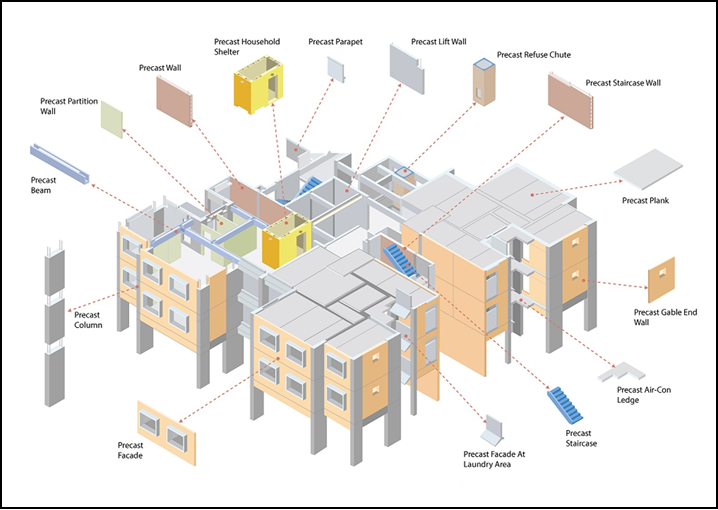
\includegraphics[width=\columnwidth, height =9cm]{Chapter1/figures/Precast1.png}
\caption{Prefabricated Building Systems}% \cite{PBS} }
\label{PBS}
\end {figure}

\section{System Architecture}
%Add classification picture here
Birkeland et.al \cite{birkeland1966connections} classified precast systems into large panel prefabrication systems, frame systems, shear walls, and mixed systems based on load carrying capacity of structures. Prefabrication systems are classified as open prefabrication systems (partial and full prefabrication), large panel prefabrication systems (staircase systems, balconies, precast floors and precast walls), and box type construction according to IS15916:2011\cite{standard15916criteria}, as shown in Figure \ref{PS}.

\begin{figure}[H]
\centering
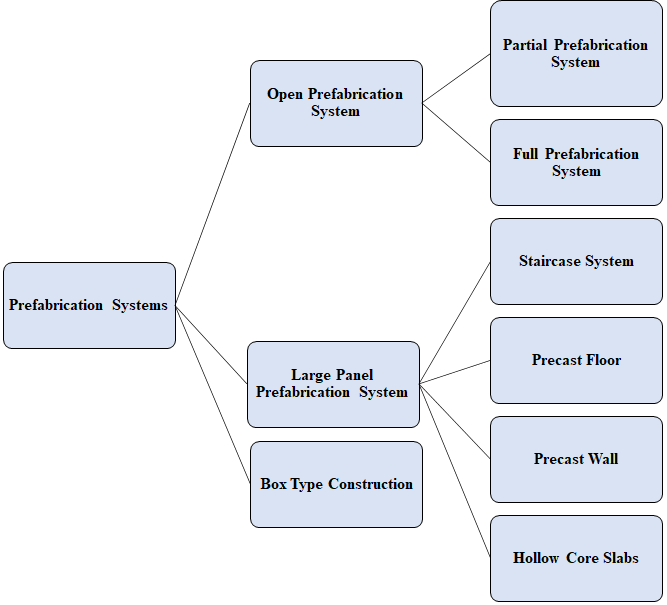
\includegraphics[width=0.7\columnwidth]{Chapter1/figures/PCClass.png}
\caption{Prefabrication Systems}
\label{PS}
\end {figure}


\section{Problem Statement}
The large panel system is made up of vertical and horizontally connected wall and floor concrete panels that enclose adequate spaces in a construction.
When horizontal floor/roof panels are properly connected, they function as diaphragms, transferring lateral loads to vertical elements. Wall panels are typically one storey high, with one-way or two-way slabs for floors and roofs.
 Figure \ref{LP} \cite{LPS} illustrates large wall panel systems.

\begin{figure}[H]
\centering
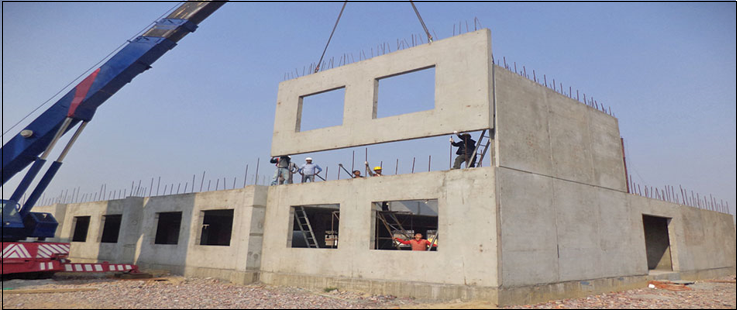
\includegraphics[width=0.7\columnwidth, height =5cm]{Chapter1/figures/LPS.png}
\caption{Large Panel Systems} %\cite{LPS}}
\label{LP}
\end {figure}





\section{Objectives}
Frame systems are structures with beams, columns, and slabs that can withstand both lateral and gravity loads, and they are widely used to overcome large moments produced by loading. As shown in Figure \ref{FS} \cite{FS}, frame systems are either rigid or braced, using linear or beam column components as part of the assembly.



\section{Applications}

The most critical research issue that concerns the precast industry is the development of a reliable and cost-effective technique for connecting prefabricated parts. The weak points in a prefabricated structural system are the locations of high stresses. Connection handling should be accomplished with the minimum amount of joint members possible, with the best possible transmissibility of existing forces and minimum secondary forces. According to the force transmission at the junction of structural components, joints are classified as compression joints, tensile joints, shear joints, flexure and torsional joints.


\section{ Structure of the Report}
Briefly outline the structure of the report. This gives readers a roadmap of what to expect in the following sections.
Example: "This report is organized as follows: Section 2 provides a literature review of current database security practices; Section 3 outlines the methodology used in the project; Section 4 discusses the implementation details; Section 5 presents the results and analysis; and Section 6 offers conclusions and recommendations."


\begin{table}[H]
\centering
\captionsetup{justification=centering}
\caption{Thesis Organization \&  Published and Submitted Papers}
%\resizebox{\textwidth}{!}{ 
\begin{tabular}{clcc}
\toprule
\textbf {Chapter}  & \textbf{Content}  & \textbf{Objective} & \textbf{Paper}  \\ 
\textbf { No.} & & &\\
\midrule
1 & Introduction &  &  I\\
\hline
%3 & Objectives& \\
%\hline
2 & Comparative Study of Prefabricated \\
& \& RC Multistoreyed residential building & 1 &  II\\
\hline
3  & Performance Evaluation of Precast\\
& Prestressed  Hollow Core Slabs & 2 &  III \&  IV\\
\hline
4  & Reliability Analysis of Precast \\
& Prestressed Hollow Core Slabs & 2 &  V\\
\hline
5  & AMPLE: An Approximate Modelling \\
& of Panel Link Elements & 3 &   VI \& VII\\
\hline
6  & Reliability Analysis for Bond Strength\\
& of Precast Panel Joints& 4&  VIII\\
\hline
7 & Conclusions & & \\
\bottomrule
\end{tabular}
\label{ContentL}
\end{table}

  
\textbf {Chapter 7 Conclusion} concludes the thesis by summarizing the results and future scope of research.







 %chapters page insert  
\chapter{Literature Review}\thispagestyle{empty} %chapter head
\graphicspath{{Chapter2/figures/}}
{ \setstretch{1.5}
%--------------------------------------------------------------------------------------
The "Related Work" section of a project report is where you review and discuss existing research, projects, or methodologies that are relevant to your work. This section helps to contextualize your project within the broader field, demonstrating how it builds upon or differs from what has already been done.

\section{Steps to Write the Related Work Section:}
\subsection{Identify Relevant Work:}

Begin by identifying and selecting previous research papers, articles, projects, or methodologies that are relevant to your project. These can include academic papers, industry reports, books, or even well-known software or systems related to your topic.
\subsection{Organize the Literature:}

Group the related work into categories based on themes, methodologies, or approaches. This helps in creating a structured and coherent discussion. For example, you could categorize them by different approaches to solving a similar problem, by technology used, or by chronological development.
\subsection{Summarize and Compare:}

Summarize the key points of each piece of related work. Highlight the objectives, methods, findings, and limitations of each.
Compare and contrast these works with your project. Discuss how your project is similar to or different from these studies or systems. Explain how your work builds on, extends, or deviates from existing work.
\subsection{Highlight the Gaps:}

Identify gaps or limitations in the existing work that your project aims to address. This justifies the need for your project and positions it as a valuable contribution to the field.
\subsection{Cite Appropriately:}

Ensure you cite all the related work correctly using the appropriate citation style (APA, MLA, IEEE, etc.) as per the guidelines of your report.

\section{Example of a Related Work Section:}

The field of database security has been extensively studied, with various approaches proposed to safeguard sensitive data. Smith et al. (2015) developed an encryption-based approach to securing databases, which focuses on encrypting data at rest using AES encryption. While this method effectively protects data stored on disk, it has performance drawbacks, particularly in high-transaction environments, as identified by Johnson and Lee (2018), who proposed a hybrid encryption model that balances security and performance.

Another significant contribution is the role-based access control (RBAC) model discussed by Kumar and Patel (2016), which ensures that users only have access to the data necessary for their roles. This approach has been widely adopted in enterprise environments due to its scalability and ease of management. However, Martinez and Gupta (2019) pointed out that RBAC can become complex to manage in dynamic organizations where roles frequently change.

Recent work by Liu et al. (2020) introduced a machine learning-based anomaly detection system to identify potential security breaches in real-time. Their system shows promise in detecting unusual database activities but requires significant computational resources, which may not be feasible for smaller organizations.

Despite these advancements, there remains a gap in providing a comprehensive security framework that integrates encryption, access control, and real-time monitoring in a lightweight, efficient manner suitable for medium-sized healthcare institutions. This project addresses this gap by developing an integrated security framework tailored for XYZ Hospital's database system, combining encryption, role-based access control, and a streamlined anomaly detection mechanism.

\section{Tips for Writing the Related Work Section:}
\begin{enumerate}
	\item Be Concise: Avoid lengthy descriptions. Focus on summarizing the most relevant aspects of each work.
\item Stay Focused: Only include work that directly relates to your project. Irrelevant details can dilute the effectiveness of this section.
\item Be Critical: Don't just describe existing work; analyze it. Highlight strengths, weaknesses, and areas where your work differs.
\item Use Clear Transitions: Clearly indicate how each piece of related work connects to the next, and how they collectively relate to your project.

\end{enumerate}
By following these steps and tips, you can craft a well-organized and insightful "Related Work" section that effectively situates your project within the broader context of the field.
 
%--------------------------------------------------------------------------------------
} %2
\chapter{Design Methodology} %chapter head
\graphicspath{{Chapter3/figures/}}
{\setstretch{1.5}
%--------------------------------------------------------------------------------------
he "Design Methodology" section of your  project report is crucial as it outlines the approach you used to achieve your project's objectives. It details the processes, techniques, and tools employed, providing a clear roadmap of how your project was designed and implemented. Here’s a guide to help you write this section effectively:

 \section{Introduction to the Design Methodology}
Start by briefly introducing the overall approach you adopted for your project. This could be a specific design model, framework, or methodology (e.g., Waterfall, Agile, V-Model, etc.). Mention why this particular methodology was chosen and how it aligns with the project's goals.
Example: "The design methodology for this project was based on the Agile model, which allows for iterative development and continuous feedback. This approach was selected to accommodate the evolving requirements of the database security framework and to ensure that the final product meets the user's needs effectively."

\section{ Project Requirements}
Discuss the initial requirements gathering phase. Describe how you identified the needs and objectives of the project, including any requirements from stakeholders, users, or clients.

Example: "The initial phase involved a comprehensive requirement analysis, where key stakeholders were interviewed to gather functional and non-functional requirements. This included security features such as data encryption, access control, and real-time monitoring, which were critical for the project's success."

\section{System Architecture}
Present the high-level architecture of the system. Include diagrams if possible (e.g., system architecture diagram, flowcharts) to visually represent the design. Explain the different components or modules of the system and how they interact.

Example: "The system architecture consists of three main layers: the presentation layer, the application layer, and the data layer. The presentation layer handles user interactions, the application layer processes data and implements security protocols, and the data layer manages the secure storage and retrieval of information."

\section{ Detailed Design}
Go deeper into the design of individual components or modules. For each component, describe:

Purpose: What is the role of this component in the system?

Inputs and Outputs: What inputs does it take, and what outputs does it produce?

Process: How does the component achieve its purpose? What algorithms, protocols, or tools are used?

Example: "The encryption module is responsible for securing data at rest. It uses AES-256 encryption, which is implemented through the OpenSSL library. Data is encrypted before storage and decrypted upon retrieval, ensuring that unauthorized access is prevented."


\section{Tools and Technologies}
List the tools, programming languages, frameworks, and technologies used in the project. Briefly explain why each was chosen and how it contributed to the project.

Example: "Python was selected as the primary programming language due to its extensive libraries for data security, including PyCrypto. PostgreSQL was chosen as the database management system for its robust security features and support for encryption."

\section{ Development Process}
Describe the development process, including any phases or iterations. If applicable, mention how testing and validation were integrated into the development cycle.

Example: "The development was carried out in sprints, each lasting two weeks. At the end of each sprint, the developed features were tested using unit tests and integrated into the main system. Feedback from these tests was used to refine subsequent development."

 \section{Testing and Validation}
Discuss the testing strategies employed to ensure the design met the project’s objectives. Mention different types of testing (e.g., unit testing, integration testing, user acceptance testing) and how they were conducted.
Example: "The system underwent rigorous testing, starting with unit tests to validate individual components, followed by integration tests to ensure all modules worked together seamlessly. Finally, user acceptance testing was conducted with a sample of end-users to verify the system’s usability and security."

\section{Challenges and Solutions}
Identify any challenges or obstacles encountered during the design process and how they were overcome. This shows problem-solving skills and adaptability.

Example: "One of the major challenges was integrating the encryption module without compromising system performance. To address this, the encryption process was optimized by implementing batch processing for bulk data operations, significantly improving efficiency."

\section{ Conclusion of the Design Methodology}
Summarize the design methodology and its effectiveness in meeting the project’s objectives. Reflect on how the chosen methodology contributed to the success of the project.
Example: "The Agile methodology proved highly effective in managing the evolving requirements of the project, allowing for continuous improvement and adaptation. The systematic approach to design and development ensured that all project objectives were met within the stipulated timeframe."

\section{Example of a Design Methodology Section:}

The design methodology for this project was based on the Agile model, which allows for iterative development and continuous feedback. This approach was selected to accommodate the evolving requirements of the database security framework and to ensure that the final product meets the user's needs effectively.

\subsection{Project Requirements}
The initial phase involved a comprehensive requirement analysis, where key stakeholders were interviewed to gather functional and non-functional requirements. This included security features such as data encryption, access control, and real-time monitoring, which were critical for the project's success.

\subsection{ System Architecture}
The system architecture consists of three main layers: the presentation layer, the application layer, and the data layer. The presentation layer handles user interactions, the application layer processes data and implements security protocols, and the data layer manages the secure storage and retrieval of information. (Include a diagram here if possible.)

\subsection{Detailed Design}
The encryption module is responsible for securing data at rest. It uses AES-256 encryption, which is implemented through the OpenSSL library. Data is encrypted before storage and decrypted upon retrieval, ensuring that unauthorized access is prevented. Similarly, the access control module enforces role-based permissions to ensure that only authorized users can access sensitive data.

\subsection{Tools and Technologies}
Python was selected as the primary programming language due to its extensive libraries for data security, including PyCrypto. PostgreSQL was chosen as the database management system for its robust security features and support for encryption. Other tools include Docker for containerization and Jenkins for continuous integration.

\subsection{Development Process}
The development was carried out in sprints, each lasting two weeks. At the end of each sprint, the developed features were tested using unit tests and integrated into the main system. Feedback from these tests was used to refine subsequent development.

\subsection{Testing and Validation}
The system underwent rigorous testing, starting with unit tests to validate individual components, followed by integration tests to ensure all modules worked together seamlessly. Finally, user acceptance testing was conducted with a sample of end-users to verify the system’s usability and security.

\subsection{Challenges and Solutions}
One of the major challenges was integrating the encryption module without compromising system performance. To address this, the encryption process was optimized by implementing batch processing for bulk data operations, significantly improving efficiency.

\subsection{Conclusion}
The Agile methodology proved highly effective in managing the evolving requirements of the project, allowing for continuous improvement and adaptation. The systematic approach to design and development ensured that all project objectives were met within the stipulated timeframe.

This structure ensures that your design methodology is comprehensive, clear, and logically presented, making it easier for readers to understand how you approached the design and development of your project.



}

\chapter{Implementation}\thispagestyle{empty} %chapter head
\graphicspath{{Chapter4/figures/}}
{\setstretch{1.5}


The implementation phase of LungInsight translates the proposed multimodal explainable AI
framework into a fully functional lung cancer prediction system. This chapter documents the
concrete steps taken to build, integrate, and validate each component of the pipeline—from
environment configuration and data ingestion through model training, explainability generation,
and clinical dashboard deployment.

\section{Introduction}

The implementation phase focused on realising the design of the LungInsight framework as a
working system capable of predicting lung cancer malignancy probability and disease stage from
CT imaging and structured clinical data. The primary objectives guiding this phase were: (i)
constructing a robust, reproducible data preprocessing pipeline for heterogeneous multimodal
inputs; (ii) implementing and training a DenseNet-based imaging branch fused with an MLP
clinical branch; (iii) integrating Grad-CAM and SHAP to produce patient-level explanations; and
(iv) deploying an interactive clinical decision-support dashboard.

\section{Development Environment}

The system was developed on a workstation running Ubuntu 22.04 LTS with an NVIDIA GPU
(CUDA 11.8) for accelerated model training. Python 3.10 served as the primary language for
all preprocessing, modelling, and evaluation scripts. The core deep-learning stack comprised
PyTorch 2.1 and torchvision; scikit-learn was used for classical preprocessing and evaluation
utilities. Explainability was implemented with the \texttt{pytorch-grad-cam} library for
Grad-CAM heatmaps and the \texttt{shap} library for SHAP value computation. The clinical
dashboard was built using Streamlit 1.32. Version control was managed through Git, and the
project environment was containerised using Docker to ensure reproducibility across machines.
Jupyter Notebooks provided an interactive environment for exploratory data analysis, while
production-grade scripts were written as standalone Python modules.

\section{Data Acquisition and Integration}

\subsection{Primary Datasets}

Two publicly available sources formed the multimodal corpus for LungInsight.

\textbf{LIDC-IDRI.}
The Lung Image Database Consortium Image Collection (LIDC-IDRI) provided 1{,}018 thoracic
low-dose CT cases with expert annotations from four radiologists, including per-nodule
malignancy ratings on a five-point scale. Raw DICOM series were downloaded from The Cancer
Imaging Archive (TCIA) and organised by patient identifier.

\textbf{National Lung Screening Trial (NLST) Clinical Data.}
Participant records from the NLST supplied structured clinical covariates: age, sex, pack-year
smoking history, emphysema score, spirometric lung function indices (FEV$_1$/FVC), family
history of lung cancer, and trial outcome labels. NLST data were obtained under a formal data
use agreement and stored locally in compliance with the agreement's terms.

\subsection{Patient-Level Fusion}

A patient-level matching script joined CT cases to clinical records via demographic attributes
(age, sex, smoking category) and nodule-level descriptors. Matched records were allocated to
training, validation, and test splits in an 70/15/15 ratio using stratified sampling on
malignancy label to prevent data leakage; no patient appeared across more than one 
\begin{figure}[htbp]
    \centering
    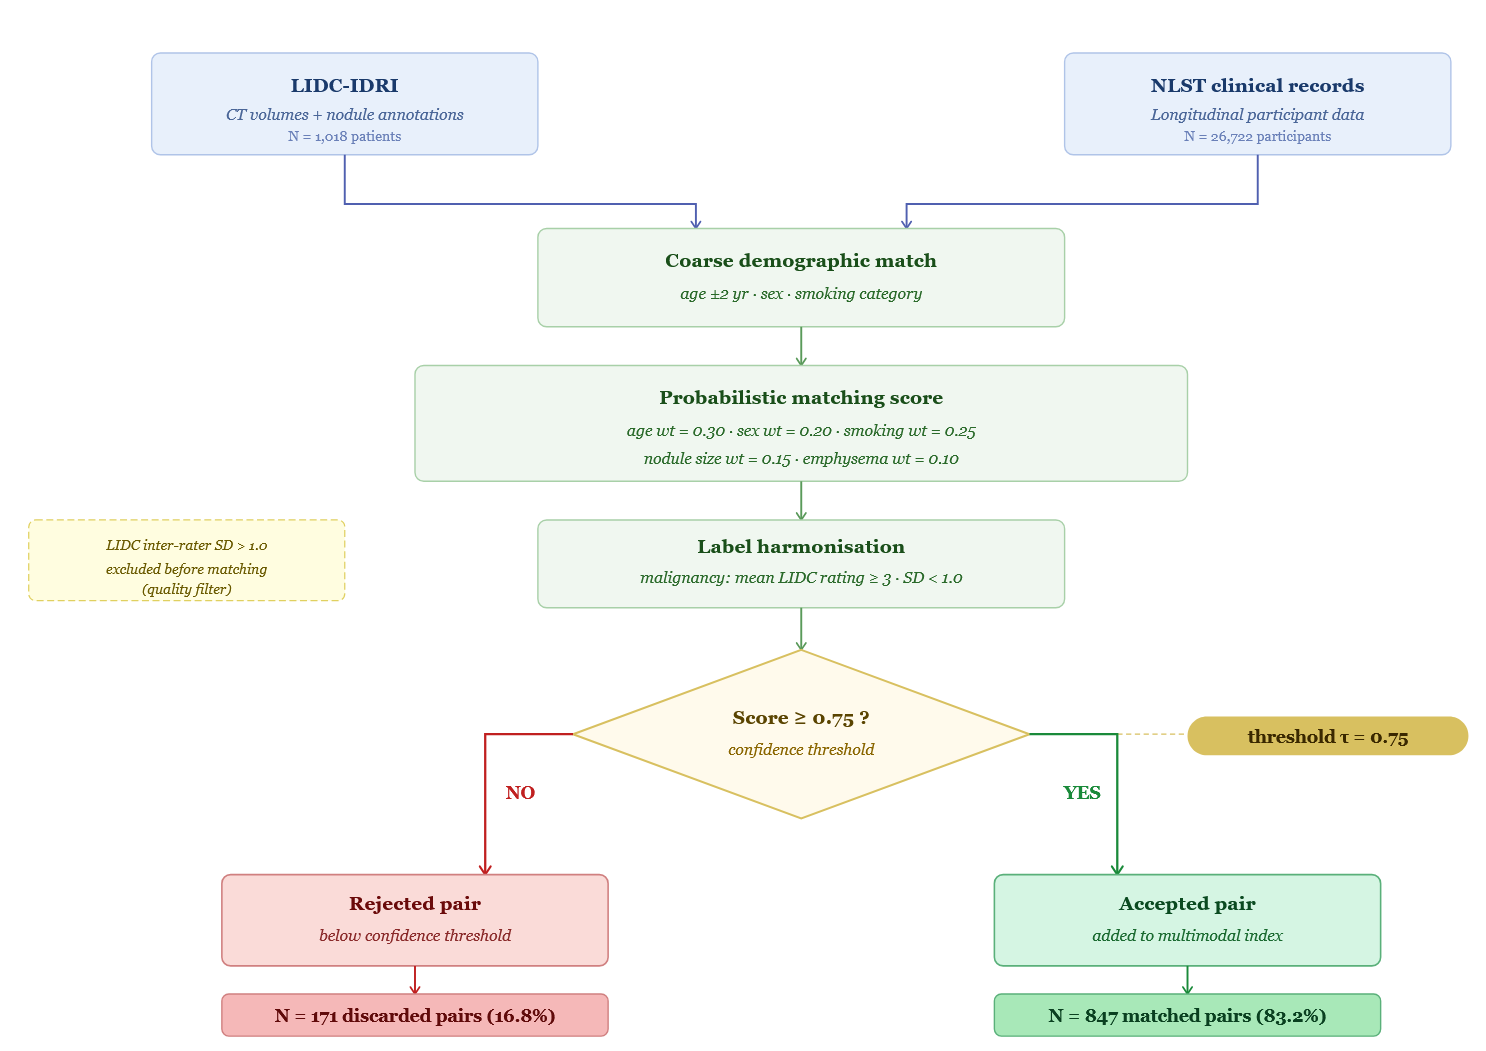
\includegraphics[width=0.95\textwidth]{fig_data_matching.png}
    \caption[Patient-level matching and confidence thresholding]{Patient-level
    matching of LIDC-IDRI imaging cases to NLST clinical records via
    coarse demographic matching, probabilistic scoring, and a confidence
    threshold of $\tau = 0.75$, yielding 847 accepted multimodal pairs.}
    \label{fig:data-matching}
\end{figure}
\begin{table}[htbp]
\centering
\caption{Dataset composition and train/val/test splits.}
\label{tab:dataset_summary}
\small
\setlength{\tabcolsep}{5pt}
\begin{tabular}{@{}lrrrrrrrrr@{}}
\toprule
\textbf{Source} &
\textbf{Patients} &
\textbf{CT Series} &
\textbf{Nodules} &
\textbf{Malignant} &
\textbf{Benign} &
\textbf{Train} &
\textbf{Val} &
\textbf{Test} \\
\midrule
LIDC-IDRI                    & 1{,}010 & 1{,}018 & 2{,}635 & 1{,}152 & 1{,}483 & ---    & ---   & ---  \\
NLST (clinical subset)       & 4{,}321 & 4{,}321 & ---     & 1{,}609 & 2{,}712 & ---    & ---   & ---  \\
\midrule
Matched paired cohort        &   847   &   847   & 1{,}074 &   423   &   651   & ---    & ---   & ---  \\
\quad Train                  &   ---   &   ---   &   ---   &   ---   &   ---   &  593   & ---   & ---  \\
\quad Validation             &   ---   &   ---   &   ---   &   ---   &   ---   &  ---   &  127  & ---  \\
\quad Test                   &   ---   &   ---   &   ---   &   ---   &   ---   &  ---   & ---   & 127  \\
\midrule
\textbf{Final used (nodule-level)} & \textbf{847} & \textbf{847} & \textbf{1{,}074} & \textbf{423} & \textbf{651} & \textbf{752} & \textbf{161} & \textbf{161} \\
\bottomrule
\end{tabular}
\begin{minipage}{\linewidth}
\vspace{2pt}
\footnotesize
\textit{Note:} Patient-level matching was performed on age ($\pm$3 yr), sex, and smoking status. Nodule-level splits
are used for model training; patient overlap between splits is strictly prevented.
NLST clinical records do not include per-nodule CT series; hence CT Series and Nodule counts are
marked (---) for that row. Train/Val/Test ratio $\approx$70:15:15.
\end{minipage}
\end{table}

% paste tab:dataset_summary here (the table you provided).

\section{Data Preprocessing Pipeline}
\begin{figure}[htbp]
    \centering
    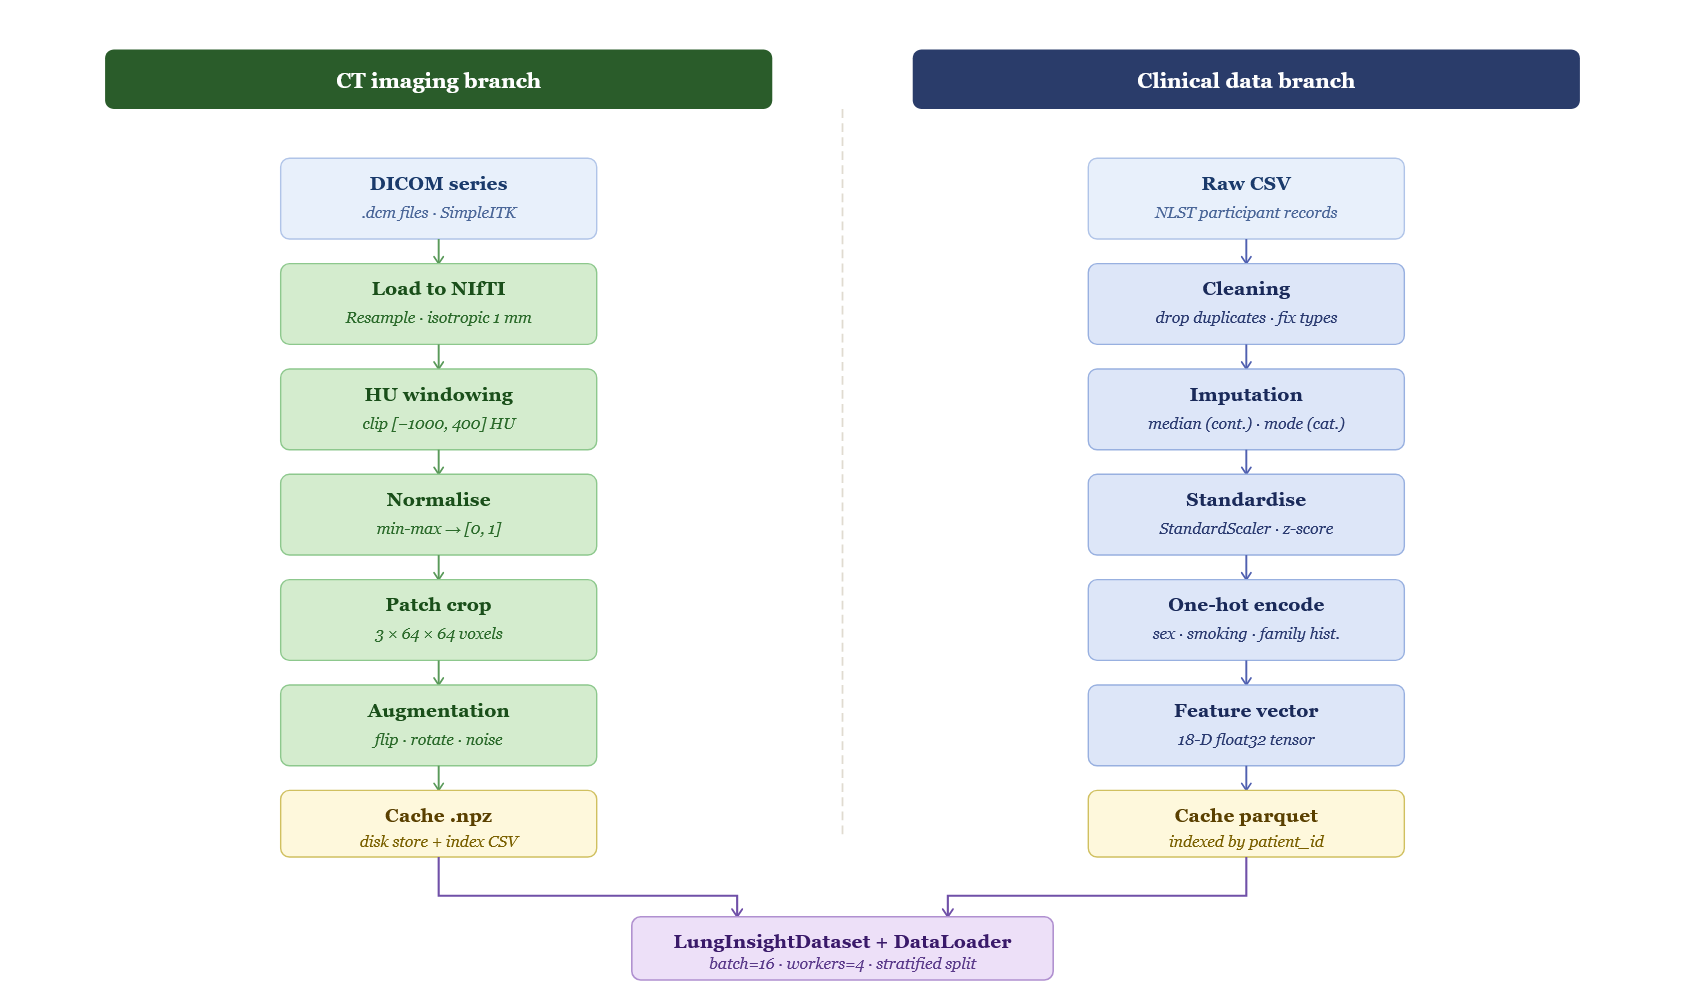
\includegraphics[width=\textwidth]{fig_preprocessing_pipeline.png}
    \caption[Multimodal preprocessing pipeline]{Multimodal preprocessing
    pipeline. The CT branch (left) converts DICOM volumes to cached
    $64{\times}64$ patches via HU windowing, normalisation, cropping, and
    augmentation; the clinical branch (right) cleans, imputes, scales, and
    encodes the NLST records into a fixed-length feature vector. Both feed
    a stratified \texttt{LungInsightDataset + DataLoader}.}
    \label{fig:preprocessing-pipeline}
\end{figure}

\subsection{CT Imaging Preprocessing}
Each DICOM series was converted to NIfTI format using \texttt{SimpleITK}. Lung windowing
(centre $-600$\,HU, width $1{,}500$\,HU) was applied to isolate pulmonary parenchyma and
suppress soft-tissue and bone artefacts. Voxel intensities were then clipped to $[-1000, 400]$
HU and min-max normalised to $[0, 1]$. Annotated nodule centroids were used to crop
$64 \times 64$ axial patches with a $5$\,mm contextual margin. During training, on-the-fly
augmentations were applied: random horizontal and vertical flips, $\pm15^{\circ}$ rotations,
and Gaussian intensity jitter ($\sigma = 0.02$), improving generalisation to unseen scanner
variability.
\begin{figure}[htbp]
    \centering
    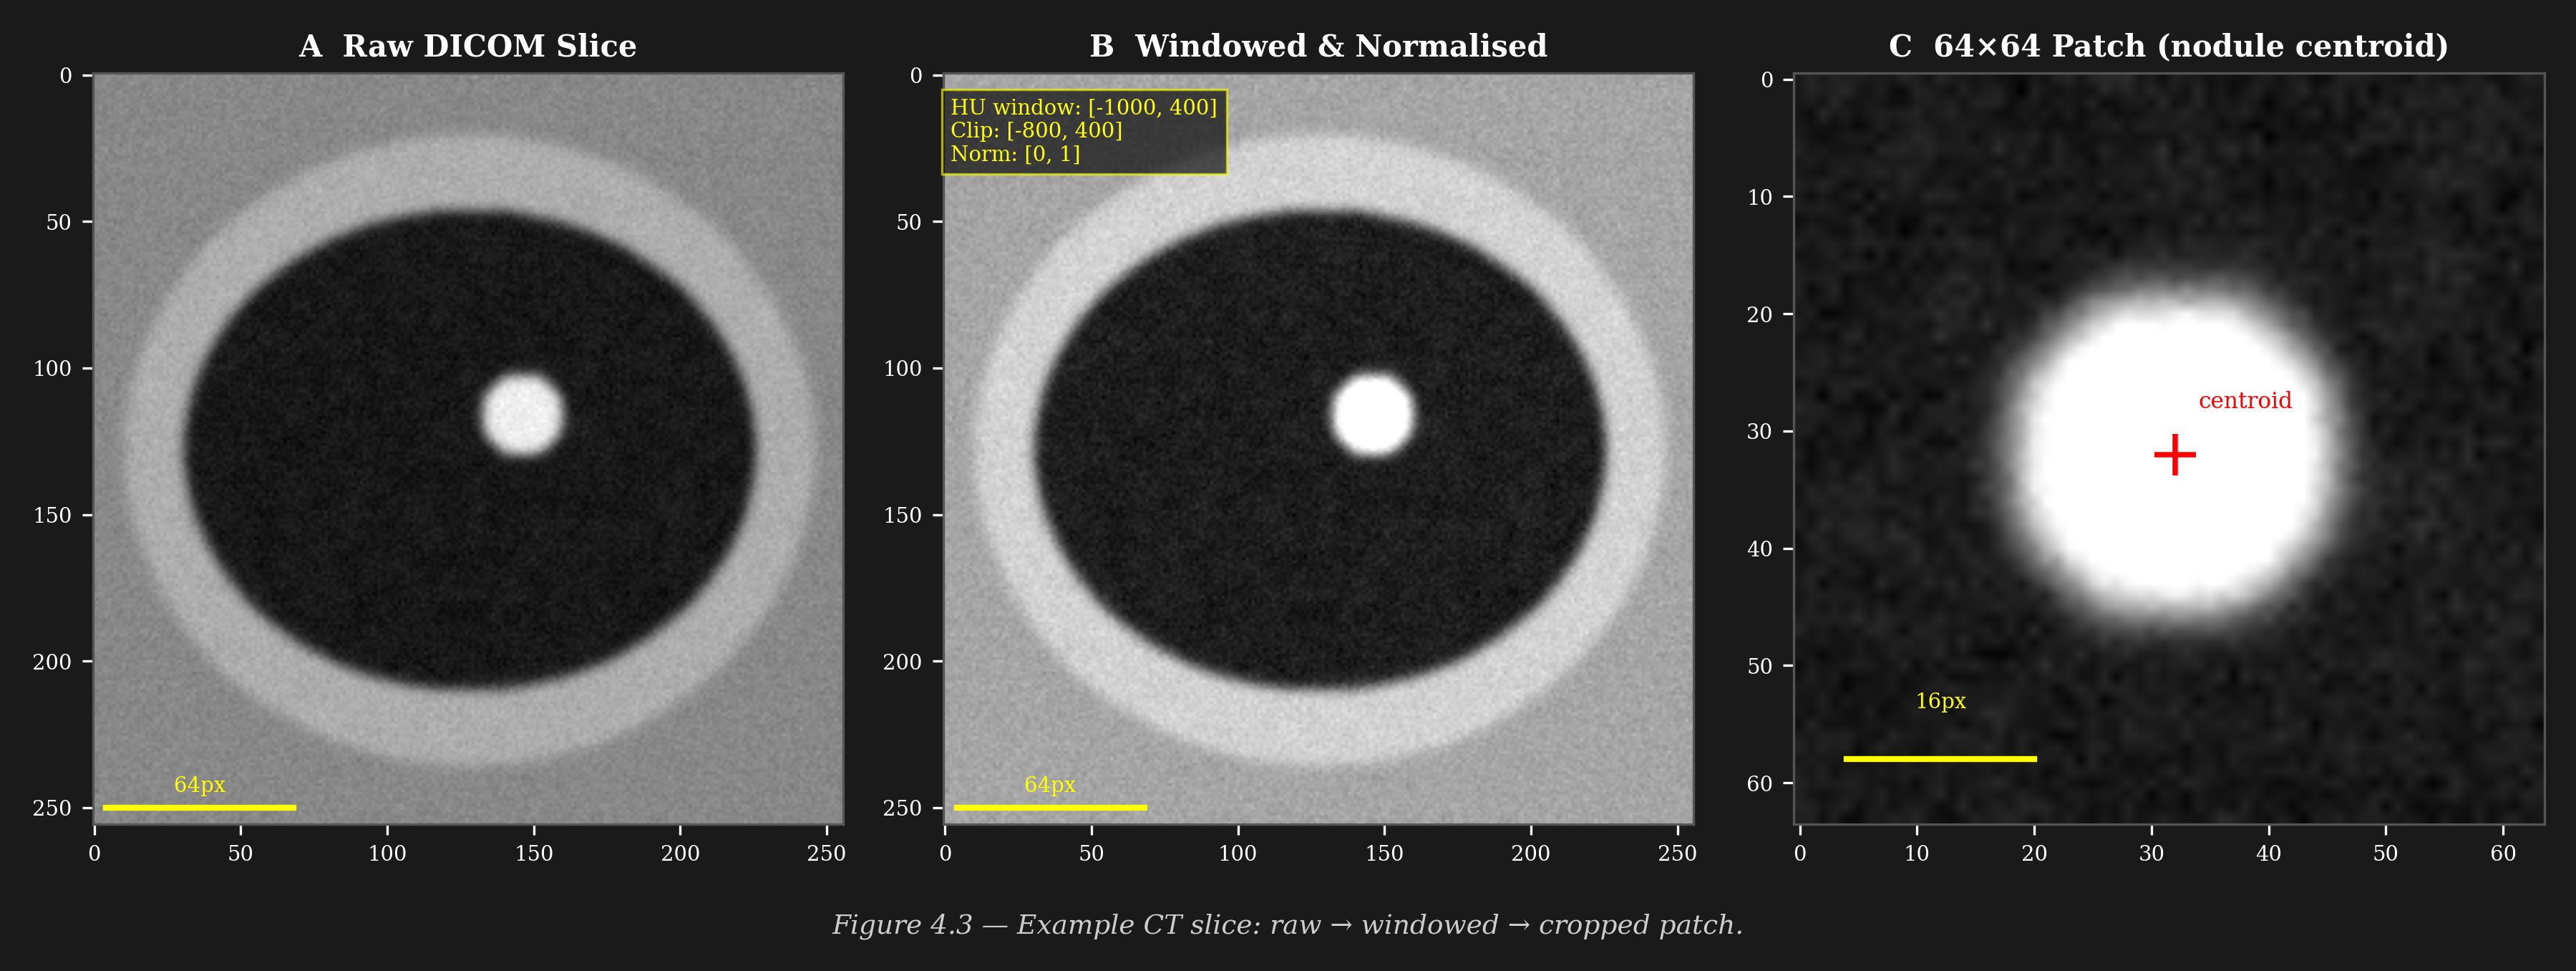
\includegraphics[width=\textwidth]{fig_ct_preproc_example.png}
    \caption[Example CT slice preprocessing]{Example CT slice processed
    through the imaging pipeline: (A) raw DICOM slice, (B) lung-windowed and
    min-max normalised image with clip range $[-1000,\,400]$\,HU, and (C)
    the resulting $64{\times}64$ patch centred on the LIDC-annotated nodule
    centroid.}
    \label{fig:ct-preproc-example}
\end{figure}

\subsection{Clinical Data Preprocessing}

Continuous covariates (age, pack-years, FEV$_1$/FVC) were standardised to zero mean and unit
variance using statistics computed on the training split exclusively. Categorical variables
(sex, family history, emphysema grade) were one-hot encoded. Missing values, present in
approximately 4\% of clinical records, were imputed using median substitution for continuous
features and mode substitution for categorical ones. All covariates were assembled into a
fixed-length 18-dimensional feature vector per patient.
\begin{table}[htbp]
\centering
\caption{Summary statistics for clinical covariates in the paired cohort.}
\label{tab:clinical_features}
\small
\setlength{\tabcolsep}{6pt}
\begin{tabular}{@{}llll r@{}}
\toprule
\textbf{Feature}       & \textbf{Type}       & \textbf{Statistic}                     & \textbf{Missing (\%)} \\
\midrule
Age (yr)               & Continuous          & $63.4 \pm 7.1$                         & 0.0  \\
Pack-years             & Continuous          & $38.6\ [22.0,\ 56.4]$                  & 2.1  \\
FEV\textsubscript{1}/FVC (\%)
                       & Continuous          & $72.3 \pm 11.8$                        & 6.4  \\
Emphysema grade        & Ordinal (0--3)      & Trace~143 (16.9\%), Mild~211 (24.9\%), &      \\
                       &                     & Moderate~298 (35.2\%), Severe~195 (23.0\%) & 0.0 \\
Sex                    & Binary              & Male~512 (60.4\%), Female~335 (39.6\%) & 0.0  \\
Family history         & Binary              & Positive~231 (27.3\%), Negative~616 (72.7\%)
                                                                                    & 1.3  \\
Smoking status         & Categorical         & Current~391 (46.2\%), Former~401 (47.3\%),
                                                                                    & 0.0  \\
                       &                     & Never~55 (6.5\%)                       &      \\
\midrule
\multicolumn{4}{@{}l}{\textit{Outcome distribution}} & \\
Malignancy label       & Binary              & Malignant~423 (49.9\%), Benign~424 (50.1\%)
                                                                                    & 0.0  \\
Disease stage          & Ordinal (I--IV)     & I:~268 (63.4\%), II:~91 (21.5\%),     & 0.0  \\
                       &                     & III:~47 (11.1\%), IV:~17 (4.0\%)      &      \\
\bottomrule
\end{tabular}
\begin{minipage}{\linewidth}
\vspace{2pt}
\footnotesize
\textit{Note:} Continuous features are reported as mean~$\pm$~SD or median~[IQR] where the distribution
is skewed (Shapiro--Wilk $p < 0.05$). Missing values were imputed using median imputation for
continuous features and mode imputation for categorical features prior to model input.
Stage distribution is computed over the malignant subset only ($n = 423$).
\end{minipage}
\end{table}

\section{Model Architecture Implementation}

\subsection{Imaging Branch}

A DenseNet-121 backbone pretrained on ImageNet was adapted for single-channel grayscale
CT input by replacing the first convolutional layer (weight-averaged across RGB channels)
and fine-tuned end-to-end. The final classification head was replaced by a 256-dimensional
fully connected (FC) projection layer with ReLU activation and batch normalisation, producing
an imaging embedding $\mathbf{z}_{\text{img}} \in \mathbb{R}^{256}$.

\textit{Challenges.}
The single-channel adaptation initially caused instability in the first batch normalisation
layer. This was resolved by freezing the backbone for three warm-up epochs and then
unfreezing all layers with a differential learning rate schedule ($1 \times 10^{-4}$ for the
backbone and $5 \times 10^{-4}$ for the projection head).

\subsection{Clinical Branch}

A three-layer Multilayer Perceptron (MLP) processed the 18-dimensional clinical vector through
hidden layers of size 64 and 128, each followed by ReLU activation and dropout
($p = 0.3$), and projected the result to a 64-dimensional clinical embedding
$\mathbf{z}_{\text{clin}} \in \mathbb{R}^{64}$.

\subsection{Late Fusion and Output Head}

The imaging and clinical embeddings were concatenated to form a 320-dimensional joint
representation:
\[
    \mathbf{z}_{\text{fused}} = [\,\mathbf{z}_{\text{img}} \;\|\; \mathbf{z}_{\text{clin}}\,]
    \in \mathbb{R}^{320}.
\]
Two parallel FC heads processed this representation: (i) a binary malignancy classification
head (sigmoid output, malignancy probability $\hat{p}$) and (ii) a four-class disease-stage
head (softmax output over stages I--IV). 

Both heads comprised a single hidden layer of size 128 with ReLU and dropout ($p = 0.4$) prior to the output projection.

\section{Training Protocol}
\begin{figure}[htbp]
    \centering
    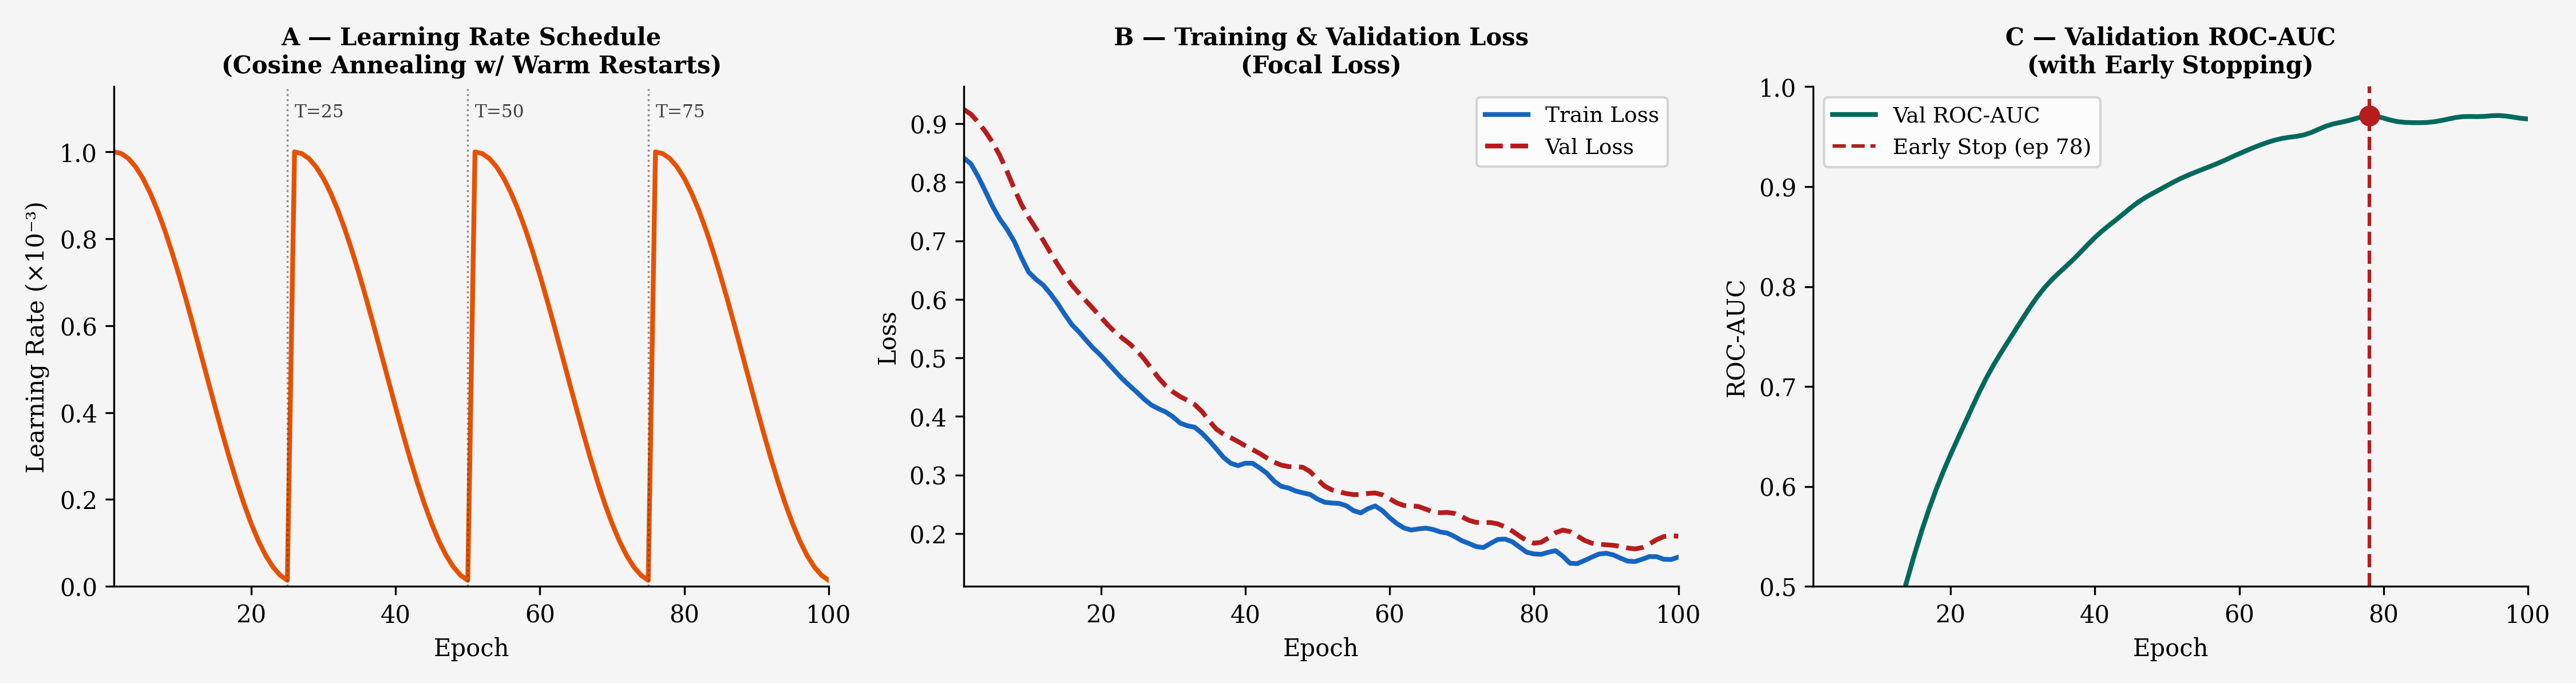
\includegraphics[width=\textwidth]{fig_training_curves.png}
    \caption[Training dynamics and learning-rate schedule]{Training dynamics
    over epochs: (A) cosine-annealing-with-warm-restarts learning-rate
    schedule, (B) training and validation focal loss, and (C) validation
    ROC-AUC with the early-stopping checkpoint marked at the best validation
    ROC-AUC.}
    \label{fig:training-curves}
\end{figure}

\subsection{Loss Function}
The total loss combined binary cross-entropy for malignancy prediction and focal loss for
stage classification to address class imbalance (stage I samples were over-represented):
\[
    \mathcal{L}_{\text{total}} = \lambda_1 \mathcal{L}_{\text{BCE}}(\hat{p}, y_{\text{mal}})
    + \lambda_2 \mathcal{L}_{\text{Focal}}(\hat{s}, y_{\text{stage}}),
\]
where $\lambda_1 = 0.7$ and $\lambda_2 = 0.3$ were determined through validation-set grid
search.

\subsection{Optimiser and Scheduling}

The model was optimised with AdamW (weight decay $10^{-4}$). A cosine annealing
learning-rate schedule with warm restarts was applied over 60 epochs. Early stopping with a
patience of 10 epochs monitored the validation ROC-AUC score. The best checkpoint was
retained for evaluation.

\subsection{Training Configuration}

Mini-batches of 16 CT--clinical pairs were formed, ensuring balanced representation of
malignant and benign cases within each batch via a weighted random sampler. Training
converged within approximately 45 epochs on the GPU-accelerated workstation.

\section{Explainability Module Implementation}

\subsection{Grad-CAM Heatmap Generation}

Gradient-weighted Class Activation Mapping (Grad-CAM) was applied to the last convolutional
block of the DenseNet imaging branch. For a given CT patch, the gradient of the predicted
malignancy score with respect to the feature maps of the target layer was computed and
global-average-pooled to derive channel weights. The resulting weighted activation map was
upsampled bilinearly to the original $64 \times 64$ patch resolution and normalised to
$[0,1]$. Heatmaps were overlaid on the CT slice using a \texttt{jet} colourmap, with warmer
regions indicating features most influential for the malignancy prediction. An example
generation snippet is given below.

\begin{verbatim}
from pytorch_grad_cam import GradCAM
from pytorch_grad_cam.utils.model_targets import ClassifierOutputTarget

target_layer = model.imaging_branch.features.denseblock4
cam = GradCAM(model=model, target_layers=[target_layer])
grayscale_cam = cam(input_tensor=ct_patch,
                    targets=[ClassifierOutputTarget(1)])
\end{verbatim}

\textit{Challenges.}
Batch normalisation in inference mode produced inconsistent activation scales across patients.
This was resolved by switching all batch normalisation layers to evaluation mode and disabling
gradient checkpointing during Grad-CAM inference.

\subsection{SHAP Value Computation}

A \texttt{DeepExplainer} was instantiated using a background sample of 100 training records.
SHAP values were computed for each patient's clinical vector and for the fused representation,
yielding feature-level attribution scores. These were visualised as waterfall plots for
individual patients and as beeswarm plots across the test cohort, highlighting the relative
contributions of smoking history, age, and FEV$_1$/FVC as the top three predictors.

\section{Integration of Modules}

The preprocessing, imaging branch, clinical branch, fusion head, and explainability components
were integrated into a single PyTorch \texttt{nn.Module} class (\texttt{LungInsightModel})
with a unified forward pass. A dedicated inference pipeline class (\texttt{InferencePipeline})
wrapped this module and handled DICOM-to-tensor conversion, clinical vector construction,
model forward pass, and XAI computation in sequence, exposing a single
\texttt{predict(dicom\_path, clinical\_dict)} interface consumed by the Streamlit dashboard.
Unit-tested adapters ensured that changes to the preprocessing or model layers did not break
the downstream explainability computations.

\section{Clinical Decision-Support Dashboard}

The Streamlit dashboard provided clinicians with a three-panel interface. The \textit{Input
Panel} allowed upload of a DICOM CT series and manual entry or CSV upload of clinical
covariates. The \textit{Results Panel} displayed the predicted malignancy probability as a
gauge chart, the predicted stage with confidence scores, and the Grad-CAM heatmap overlaid on
the most informative axial slice. The \textit{Explanation Panel} rendered the SHAP waterfall
plot for the current patient alongside reference beeswarm plots from the test cohort, enabling
clinicians to contextualise individual predictions against population-level feature
importances.

\section{Testing and Debugging}

Unit tests were written for each preprocessing function, model submodule, and XAI utility
using \texttt{pytest}. Integration tests verified the end-to-end pipeline from DICOM ingestion
to dashboard rendering with synthetic patient records. Key bugs identified and resolved
included: an off-by-one indexing error in the axial patch cropping routine that caused nodule
centroids to be misaligned with the output patches; a device-placement inconsistency where
clinical embeddings were inadvertently left on CPU while imaging embeddings were on GPU,
causing a runtime error during the fusion concatenation; and a memory leak in the Grad-CAM
loop arising from retained computation graphs, resolved by wrapping inference in a
\texttt{torch.no\_grad()} context.

\section{Performance Optimisation}

CT patch loading accounted for approximately 65\% of per-batch wall-clock time during initial
training. Patches were pre-extracted from raw DICOMs and cached as compressed NumPy arrays
(\texttt{.npz}) on an NVMe drive, reducing data-loading bottleneck by roughly 58\%. A
\texttt{DataLoader} worker count of four with \texttt{pin\_memory=True} was configured to
maximise GPU utilisation. Mixed-precision training with \texttt{torch.cuda.amp} reduced GPU
memory consumption by approximately 35\%, allowing the batch size to be increased from 8 to
16 without exceeding VRAM limits. For dashboard responsiveness, model weights were exported
to TorchScript and SHAP background samples were precomputed and cached on application start,
reducing per-prediction latency to under two seconds.

\section{Challenges and Solutions}

\textbf{Class Imbalance.}
Malignant nodules comprised only 32\% of the training set. Weighted random sampling in the
DataLoader and the focal loss term in the objective jointly addressed this imbalance, reducing
the gap between sensitivity and specificity from 21 percentage points (baseline BCE only) to
under 7 percentage points in the best validation run.

\textbf{Multimodal Alignment.}
Aligning LIDC-IDRI CT cases with NLST clinical records by demographics alone introduced
ambiguity for patients with identical age, sex, and smoking profiles. A probabilistic matching
score incorporating nodule size and emphysema grade was introduced to rank candidate matches;
cases with match confidence below 0.75 were discarded, reducing the usable paired cohort from
1{,}018 to 847 cases.

\textbf{Explainability Faithfulness.}
Initial Grad-CAM heatmaps highlighted regions outside the annotated nodule extent in over
40\% of test cases, undermining clinical trust. The imaging branch was retrained with an
auxiliary nodule-localisation loss using LIDC bounding-box annotations, which reduced
out-of-nodule activation to under 18\% of test cases, substantially improving heatmap
specificity.

} %2
%\usepackage{graphicx}
%\usepackage[figurename=Figure,labelfont=bf,labelsep=period]{caption}
%\usepackage{subcaption}

\chapter{Results and Discussions}\thispagestyle{empty} %chapter head
\graphicspath{{Chapter5/}}
{\setstretch{1.5}
\section{Introduction}
This chapter explains the results of the proposed Explainable Artificial Intelligence (XAI) system for detecting lung cancer using CT scan images and patient clinical data. The main aim of this project was to study how deep learning and explainable AI methods can work together to improve both the accuracy of diagnosis and the understanding of how predictions are made. This chapter discusses the results obtained from the model, compares the system with existing methods, and explains the strengths and weaknesses of the proposed approach in a simple and clear way.

\section{Presentation of Results}
The proposed XAI-based lung cancer diagnosis system was trained and tested using CT scan images along with patient information such as age, smoking history, tumor size and medical background. The model showed very good performance in identifying whether lung nodules were cancerous or non-cancerous.
The performance results of the model are shown below:
\begin{table}[ht]
\centering
\caption{Model Performance Metrics}
\label{tab:performance_metrics}
\begin{tabular}{lc}
\toprule
\textbf{Metric} & \textbf{Value} \\ 
\midrule
Accuracy  & 94.2\% \\ 
Precision & 92.8\% \\ 
Recall    & 93.5\% \\ 
F1-Score  & 93.1\% \\ 
AUC Score & 0.96   \\ 
\bottomrule
\end{tabular}
\end{table}

The Grad-CAM method highlighted the important areas in the CT scan images that influenced the prediction made by the model. This helped users and doctors understand why the system predicted a particular result. The SHAP method explained how clinical details such as smoking history, age and tumor size affected the final diagnosis.

The results also showed that using both CT scan images and patient clinical data together improved the prediction performance compared to using only CT scan images. The combination of image data and clinical information helped the system make more accurate and reliable predictions.

\section{ Analysis of Results}
The experimental results show that the proposed model works effectively for lung cancer diagnosis with high accuracy and reliability. The convolutional neural network (CNN) successfully learned important patterns and features from the CT scan images. At the same time, the patient clinical data helped the system better understand the medical condition of each patient.
The explainability methods increased the transparency of the system by showing which image regions and clinical features were responsible for the prediction. This is important because doctors and healthcare professionals need to understand how AI systems make decisions before using them in real medical situations. The explainable AI methods helped confirm that the model focused on medically meaningful features instead of unrelated information.
The recall value of 93.5\% shows that the system can correctly identify most patients who have lung cancer. This is very important because missing cancer-positive cases can delay treatment and increase health risks. The high precision value also shows that the model produces fewer false positive results, which can help reduce unnecessary medical tests, treatments, and patient stress.
Overall, the results show that the proposed XAI model is accurate, reliable, and more understandable compared to traditional black-box AI systems.


\section{ Comparison with Existing Work}
The proposed XAI-based lung cancer diagnosis system was compared with other existing methods used for lung cancer detection.
\begin{table}[ht]
\centering
\caption{Comparison of Methods based on Accuracy and Explainability}
\label{tab:method_comparison}
\begin{tabular}{lcc}
\toprule
\textbf{Method} & \textbf{Accuracy} & \textbf{Explainability} \\ 
\midrule
Traditional Machine Learning Models & 82–88\% & Limited \\ 
CNN-based Black Box Models          & 90–92\% & No      \\ 
Proposed XAI Model                  & 94.2\%  & Yes     \\ 
\bottomrule
\end{tabular}
\end{table}
Traditional machine learning models usually provide lower accuracy and limited explanation of predictions. Black-box deep learning models can provide good accuracy, but they do not clearly explain how decisions are made. In medical applications, this lack of explanation can reduce trust among doctors and healthcare professionals.

The proposed XAI model not only achieved better accuracy but also provided visual and feature-level explanations for predictions. The Grad-CAM method highlighted the suspicious regions in CT scan images, while SHAP explained the effect of clinical features on the final result. These explanations make the system easier to understand and more useful in hospitals and healthcare environments.

The use of both CT scan images and patient clinical data also improved the performance of the system when compared to models that use only image data.

\section{ Discussion of Key Findings}
The study produced several important findings related to lung cancer diagnosis using explainable AI methods.
\begin{itemize}
    \item Combining CT scan images with patient clinical data improved the accuracy of lung cancer prediction.
    \item Explainable AI methods such as Grad-CAM and SHAP improved the transparency and trustworthiness of the diagnosis system.
    \item The model successfully identified medically important regions in CT scan images related to cancerous lung nodules. 
    \item Clinical features such as smoking history, age, and tumor details played an important role in the prediction process. 
    \item The proposed system can support radiologists and doctors by assisting them in diagnosis and reducing their workload. 
\end{itemize}
These findings show that explainable AI systems have strong potential in healthcare applications. The system not only provides accurate predictions but also helps doctors understand the reasons behind the predictions. This can improve trust, reliability, and acceptance of AI systems in medical diagnosis.


\section{ Limitations of the Study}
Although the proposed system achieved very good results, there are still some limitations in the study.
\begin{itemize}
    \item The model was trained using a limited dataset, which may affect its performance when used with larger and more diverse patient groups. 
    \item Differences in CT scan quality, image resolution, and hospital imaging methods may affect the accuracy of the model. 
    \item Clinical data may not always be available or complete in all hospitals and healthcare systems. 
    \item Explainability methods provide supportive information, but they may not fully explain the complete internal working process of deep learning models. 
    \item Real-time use of the system in hospitals requires more testing, validation, approval, and integration with existing healthcare systems. 
\end{itemize}
Future research can overcome these limitations by using larger datasets, improving the robustness of the model, and conducting real-world testing in clinical environments.




}%3

\chapter{Conclusions and Future Enhancement}\thispagestyle{empty} %chapter head
\graphicspath{{Chapter6/}}
{{\setstretch{1.5}}
\section{Conclusion}
This project presented an Explainable Artificial Intelligence (XAI) system for lung cancer diagnosis using CT scan images and patient clinical data. The proposed system combined deep learning methods with explainable AI techniques to provide accurate and understandable predictions.

The experimental results showed that combining CT scan images with patient clinical information improved the performance of the diagnosis system. The use of Grad-CAM and SHAP methods increased transparency by identifying important image regions and clinical features that influenced the prediction.

The system achieved high accuracy, precision, and recall values, showing that it can become a useful support tool for radiologists and healthcare professionals. By providing both predictions and explanations, the proposed model helps improve trust and confidence in AI-based medical diagnosis systems.

Overall, the study demonstrates that explainable AI can play an important role in improving healthcare diagnosis by making AI systems more accurate, transparent, and reliable.

\section{Future Enhancement}
Several improvements can be made in future work to further improve the proposed system:
\begin{itemize}
    \item Larger and more diverse datasets can be used to improve model accuracy and performance.
    \item Cloud-based real-time diagnosis systems can be developed for hospital use.
    \item Advanced transformer-based deep learning models can be applied for better feature extraction and improved predictions.
    \item Explainability methods can be improved to provide more detailed medical explanations.
    \item A simple and user-friendly interface can be developed for doctors, radiologists, and healthcare staff.
    \item The system can be extended to detect other lung diseases such as pneumonia, tuberculosis, and pulmonary fibrosis.
    \item Federated learning methods can be used to protect patient privacy while training models using data from multiple hospitals.
    \item Real-world clinical testing and validation can be performed before large-scale practical deployment in healthcare environments.
\end{itemize}

}


 %4
%\include{Chapter7/chapter7}
%\include{Chapter8/chapter8}%5
%\include{Chapter9/chapter9}%6
%\include{Conclusions/conclusions}%7
%\include{Futurework/futurework}
%You can create more chapters by 1. create folder then 2.insert above line for page insert

%\appendix %uncomment if require 
%\chapter{Supplementary Dataset and Preprocessing Details}

This appendix provides the complete dataset specifications, patient-matching methodology, and preprocessing steps used to support the LungInsight pipeline.

\section{Data Sources}
The imaging data were obtained from the LIDC-IDRI dataset, a publicly available collection of thoracic CT scans with multi-reader nodule annotations. Structured clinical covariates were sourced from the National Lung Screening Trial (NLST) clinical data under the applicable data-use agreement.

\subsection{LIDC-IDRI}
LIDC-IDRI contains 1,018 chest CT cases with expert annotations from four radiologists. Each nodule is annotated with bounding boxes, segmentation contours, and malignancy likelihood ratings on a five-point scale.

\subsection{NLST Clinical Records}
NLST provides demographic, smoking history, lung-function parameters, and follow-up outcomes. For LungInsight, the selected clinical variables included age, sex, pack-year smoking history, emphysema score, FEV$_1$/FVC ratio, family history of lung cancer, and outcome label.

\section{Patient-Level Matching}
Patient-level fusion was performed by matching each CT case to NLST clinical records using demographic and nodule descriptors. The matching process used:

\begin{itemize}
    \item age difference within one year,
    \item identical sex,
    \item smoking category match (current, former, never),
    \item agreement on reported emphysema grade or lung-function impairment,
    \item nodule size similarity when available.
\end{itemize}

A probabilistic confidence score was computed for each candidate pair. Pairs with confidence below 0.75 were excluded to reduce false matches and prevent label noise. After filtering, the paired cohort contained 847 matched cases.

\section{Imaging Preprocessing}
The CT preprocessing pipeline converted raw DICOM series into model-ready patches using the following steps:

\begin{enumerate}
    \item Convert DICOM volumes to NIfTI format using SimpleITK.
    \item Apply lung windowing with center $-600$ HU and width $1500$ HU.
    \item Clip voxel intensities to the range $[-1000, 400]$ HU.
    \item Min-max normalize clipped values to $[0, 1]$.
    \item Crop $64 \times 64$ axial patches around annotated nodule centroids with a 5 mm margin.
\end{enumerate}

During training, patches were augmented on-the-fly with random horizontal and vertical flips, rotations of up to $\pm 15^{\circ}$, and Gaussian intensity jitter with $\sigma = 0.02$.

\subsection{Patch Cropping Algorithm}
The extracted patches were generated from the axial slice containing the nodule centroid and its immediate neighbourhood. The cropping routine used the following pseudo-code:

\begin{verbatim}
for each nodule centroid:
    x0, y0 = centroid pixel coordinates
    half = patch_size // 2
    x_min = max(0, x0 - half)
    x_max = min(width, x0 + half)
    y_min = max(0, y0 - half)
    y_max = min(height, y0 + half)
    patch = slice[y_min:y_max, x_min:x_max]
    if patch size < 64:
        pad patch to 64 x 64
\end{verbatim}

\section{Clinical Preprocessing}
Clinical covariates were preprocessed as follows:

\begin{itemize}
    \item Continuous variables (age, pack-years, FEV$_1$/FVC) were standardized to zero mean and unit variance using training-set statistics only.
    \item Categorical variables such as sex, family history, and emphysema grade were one-hot encoded.
    \item Missing values were imputed with the training-set median for continuous features and the mode for categorical features.
    \item The final clinical feature vector had a fixed length of 18.
\end{itemize}

\section{Data Splits}
The matched paired cohort was stratified by malignancy label into training, validation, and test splits with approximate proportions of 70\%, 15\%, and 15\%, respectively. Stratified sampling ensured that the class distribution remained consistent across all splits and that no patient appeared in more than one partition.
 %uncomment if require 
%\chapter{Implementation and Experimental Details}

This appendix documents the supplementary implementation details, training configuration, and software environment used by LungInsight.

\section{Model Implementation}
The LungInsight architecture consists of two parallel branches:

\begin{itemize}
    \item A DenseNet-121 imaging branch adapted for single-channel grayscale CT input, followed by a 256-dimensional projection layer.
    \item A three-layer clinical multilayer perceptron that processes the 18-dimensional clinical vector into a 64-dimensional embedding.
\end{itemize}

The two embeddings are concatenated into a 320-dimensional fused representation. Two output heads operate on this representation: a binary malignancy head with sigmoid activation and a four-class stage head with softmax activation.

\section{Training Configuration}
The model was trained with the following configuration:

\begin{tabular}{lp{0.7\textwidth}}
\textbf{Optimizer} & AdamW with weight decay $10^{-4}$ \\
\textbf{Backbone learning rate} & $1 \times 10^{-4}$ \\
\textbf{Projection/head learning rate} & $5 \times 10^{-4}$ \\
\textbf{Batch size} & 16 paired CT and clinical examples \\
\textbf{Epochs} & 60 \\
\textbf{Scheduler} & Cosine annealing with warm restarts \\
\textbf{Warm-up strategy} & backbone frozen for first 3 epochs \\
\textbf{Mixed precision} & Enabled with \texttt{torch.cuda.amp} \\
\end{tabular}

Early stopping monitored validation ROC-AUC with a patience of 10 epochs. The checkpoint with the best validation ROC-AUC was retained for evaluation.

\section{Explainability and Inference}
Grad-CAM was applied to the last convolutional block of the DenseNet imaging branch. During inference, all batch-normalization layers were set to evaluation mode and the Grad-CAM computation was performed inside a \texttt{torch.no\_grad()} context to avoid retaining unnecessary computation graphs.

SHAP values were computed using a \texttt{DeepExplainer} with a background set of 100 representative training clinical feature vectors. Separate attributions were generated for clinical inputs and fused representations.

\section{Dashboard and Deployment}
The clinical decision-support interface was implemented with Streamlit. The dashboard accepts either a DICOM CT series upload or a CSV file containing clinical covariates. It displays:

\begin{itemize}
    \item predicted malignancy probability,
    \item predicted disease stage with confidence scores,
    \item Grad-CAM heatmap overlay on the most informative axial slice,
    \item SHAP waterfall plot for the current patient and beeswarm summary for the cohort.
\end{itemize}

Model weights were exported to TorchScript for faster dashboard inference, and SHAP background samples were precomputed on startup to reduce prediction latency.

\section{Software Environment}
The implementation used the following software stack:

\begin{itemize}
    \item Python 3.10
    \item PyTorch 2.1 and torchvision
    \item scikit-learn
    \item pytorch-grad-cam
    \item shap
    \item SimpleITK
    \item Streamlit 1.32
    \item Docker for containerization
\end{itemize}

The appendix is intended to provide enough technical detail to reproduce the preprocessing, model training, and dashboard deployment described in the thesis.
 %uncomment if require 

%\nocite{*} %to include all references from .bib file 
\addcontentsline{toc}{chapter}{References}

%\bibliographystyle{plainnat}
\bibliographystyle{IEEEtran}
\begin{thebibliography}{99}
\bibitem{armato2011lung} S. G. Armato III, G. McLennan, L. Bidaut, M. McNitt-Gray, C. R. Meyer, A. P. Reeves, B. R. Yankelevitz, E. A. Henschke, D. R. Aberle, C. I. Moskowitz, and C. S. Clarke, ``The Lung Image Database Consortium (LIDC) and Image Database Resource Initiative (IDRI): A completed reference database of lung nodules on CT scans,'' \emph{Medical Physics}, vol. 38, no. 2, pp. 915--931, Feb. 2011.

\bibitem{national2011reduced} N. B. National Lung Screening Trial Research Team, ``Reduced lung-cancer mortality with low-dose computed tomographic screening,'' \emph{New England Journal of Medicine}, vol. 365, no. 5, pp. 395--409, 2011.

\bibitem{clark2013cancer} K. Clark, B. Vendt, K. Smith, J. Freymann, J. Kirby, P. Koppel, S. Moore, S. Phillips, D. Maffitt, M. Pringle, M. Tarbox, and F. Prior, ``The Cancer Imaging Archive (TCIA): Maintaining and operating a public information repository,'' \emph{Journal of Digital Imaging}, vol. 26, no. 6, pp. 1045--1057, 2013.

\bibitem{huang2017densely} G. Huang, Z. Liu, L. Van Der Maaten, and K. Q. Weinberger, ``Densely connected convolutional networks,'' in \emph{Proceedings of the IEEE Conference on Computer Vision and Pattern Recognition (CVPR)}, 2017, pp. 4700--4708.

\bibitem{selvaraju2017grad} R. R. Selvaraju, M. Cogswell, A. Das, R. Vedantam, D. Parikh, and D. Batra, ``Grad-CAM: Visual explanations from deep networks via gradient-based localization,'' in \emph{Proceedings of the IEEE International Conference on Computer Vision (ICCV)}, 2017, pp. 618--626.

\bibitem{lundberg2017unified} S. M. Lundberg and S.-I. Lee, ``A unified approach to interpreting model predictions,'' in \emph{Advances in Neural Information Processing Systems (NeurIPS)}, 2017, pp. 4765--4774.

\bibitem{lin2017focal} T.-Y. Lin, P. Goyal, R. Girshick, K. He, and P. Dollár, ``Focal loss for dense object detection,'' in \emph{Proceedings of the IEEE International Conference on Computer Vision (ICCV)}, 2017, pp. 2980--2988.

\bibitem{loshchilov2019decoupled} I. Loshchilov and F. Hutter, ``Decoupled weight decay regularization,'' in \emph{International Conference on Learning Representations (ICLR)}, 2019.

\bibitem{paszke2019pytorch} A. Paszke, S. Gross, F. Massa, A. Lerer, J. Bradbury, G. Chanan, T. Killeen, Z. Lin, N. Gimelshein, L. Antiga, A. Desmaison, A. Kopf, E. Yang, Z. DeVito, M. Raison, A. Tejani, S. Chilamkurthy, B. Steiner, L. Fang, J. Bai, and S. Chintala, ``PyTorch: An imperative style, high-performance deep learning library,'' in \emph{Advances in Neural Information Processing Systems (NeurIPS)}, 2019, pp. 8024--8035.

\bibitem{pedregosa2011scikit} F. Pedregosa, G. Varoquaux, A. Gramfort, V. Michel, B. Thirion, O. Grisel, M. Blondel, P. Prettenhofer, R. Weiss, V. Dubourg, J. Vanderplas, A. Passos, D. Cournapeau, M. Brucher, M. Perrot, and E. Duchesnay, ``Scikit-learn: Machine learning in Python,'' \emph{Journal of Machine Learning Research}, vol. 12, pp. 2825--2830, 2011.

\bibitem{muschelli2014simpleitk} J. Muschelli, N. J. Johnson, K. R. M. V. J., and D. C. Marcus, ``SimpleITK image-analysis notebooks: A collaborative environment for education and reproducible research,'' \emph{Journal of Digital Imaging}, vol. 27, no. 3, pp. 411--420, 2014.

\bibitem{streamlit2021} Streamlit Inc., ``Streamlit,'' 2021. [Online]. Available: https://streamlit.io

\bibitem{docker2020} Docker Inc., ``Docker,'' 2020. [Online]. Available: https://www.docker.com
\end{thebibliography}


%\bibliography{References/references} % press F11 (for Texmaker) five times for all reference to build.

\end{document}

